% Options for packages loaded elsewhere
\PassOptionsToPackage{unicode}{hyperref}
\PassOptionsToPackage{hyphens}{url}
\PassOptionsToPackage{dvipsnames,svgnames,x11names}{xcolor}
%
\documentclass[
  11pt,
]{article}

\usepackage{amsmath,amssymb}
\usepackage{iftex}
\ifPDFTeX
  \usepackage[T1]{fontenc}
  \usepackage[utf8]{inputenc}
  \usepackage{textcomp} % provide euro and other symbols
\else % if luatex or xetex
  \usepackage{unicode-math}
  \defaultfontfeatures{Scale=MatchLowercase}
  \defaultfontfeatures[\rmfamily]{Ligatures=TeX,Scale=1}
\fi
\usepackage{lmodern}
\ifPDFTeX\else  
    % xetex/luatex font selection
\fi
% Use upquote if available, for straight quotes in verbatim environments
\IfFileExists{upquote.sty}{\usepackage{upquote}}{}
\IfFileExists{microtype.sty}{% use microtype if available
  \usepackage[]{microtype}
  \UseMicrotypeSet[protrusion]{basicmath} % disable protrusion for tt fonts
}{}
\makeatletter
\@ifundefined{KOMAClassName}{% if non-KOMA class
  \IfFileExists{parskip.sty}{%
    \usepackage{parskip}
  }{% else
    \setlength{\parindent}{0pt}
    \setlength{\parskip}{6pt plus 2pt minus 1pt}}
}{% if KOMA class
  \KOMAoptions{parskip=half}}
\makeatother
\usepackage{xcolor}
\usepackage[lmargin=1in,rmargin=1in,tmargin=1in,bmargin=1in]{geometry}
\setlength{\emergencystretch}{3em} % prevent overfull lines
\setcounter{secnumdepth}{3}
% Make \paragraph and \subparagraph free-standing
\ifx\paragraph\undefined\else
  \let\oldparagraph\paragraph
  \renewcommand{\paragraph}[1]{\oldparagraph{#1}\mbox{}}
\fi
\ifx\subparagraph\undefined\else
  \let\oldsubparagraph\subparagraph
  \renewcommand{\subparagraph}[1]{\oldsubparagraph{#1}\mbox{}}
\fi


\providecommand{\tightlist}{%
  \setlength{\itemsep}{0pt}\setlength{\parskip}{0pt}}\usepackage{longtable,booktabs,array}
\usepackage{calc} % for calculating minipage widths
% Correct order of tables after \paragraph or \subparagraph
\usepackage{etoolbox}
\makeatletter
\patchcmd\longtable{\par}{\if@noskipsec\mbox{}\fi\par}{}{}
\makeatother
% Allow footnotes in longtable head/foot
\IfFileExists{footnotehyper.sty}{\usepackage{footnotehyper}}{\usepackage{footnote}}
\makesavenoteenv{longtable}
\usepackage{graphicx}
\makeatletter
\def\maxwidth{\ifdim\Gin@nat@width>\linewidth\linewidth\else\Gin@nat@width\fi}
\def\maxheight{\ifdim\Gin@nat@height>\textheight\textheight\else\Gin@nat@height\fi}
\makeatother
% Scale images if necessary, so that they will not overflow the page
% margins by default, and it is still possible to overwrite the defaults
% using explicit options in \includegraphics[width, height, ...]{}
\setkeys{Gin}{width=\maxwidth,height=\maxheight,keepaspectratio}
% Set default figure placement to htbp
\makeatletter
\def\fps@figure{htbp}
\makeatother
% definitions for citeproc citations
\NewDocumentCommand\citeproctext{}{}
\NewDocumentCommand\citeproc{mm}{%
  \begingroup\def\citeproctext{#2}\cite{#1}\endgroup}
\makeatletter
 % allow citations to break across lines
 \let\@cite@ofmt\@firstofone
 % avoid brackets around text for \cite:
 \def\@biblabel#1{}
 \def\@cite#1#2{{#1\if@tempswa , #2\fi}}
\makeatother
\newlength{\cslhangindent}
\setlength{\cslhangindent}{1.5em}
\newlength{\csllabelwidth}
\setlength{\csllabelwidth}{3em}
\newenvironment{CSLReferences}[2] % #1 hanging-indent, #2 entry-spacing
 {\begin{list}{}{%
  \setlength{\itemindent}{0pt}
  \setlength{\leftmargin}{0pt}
  \setlength{\parsep}{0pt}
  % turn on hanging indent if param 1 is 1
  \ifodd #1
   \setlength{\leftmargin}{\cslhangindent}
   \setlength{\itemindent}{-1\cslhangindent}
  \fi
  % set entry spacing
  \setlength{\itemsep}{#2\baselineskip}}}
 {\end{list}}
\usepackage{calc}
\newcommand{\CSLBlock}[1]{\hfill\break\parbox[t]{\linewidth}{\strut\ignorespaces#1\strut}}
\newcommand{\CSLLeftMargin}[1]{\parbox[t]{\csllabelwidth}{\strut#1\strut}}
\newcommand{\CSLRightInline}[1]{\parbox[t]{\linewidth - \csllabelwidth}{\strut#1\strut}}
\newcommand{\CSLIndent}[1]{\hspace{\cslhangindent}#1}

\makeatletter
\@ifpackageloaded{float}{}{\usepackage{float}}
\floatstyle{plain}
\@ifundefined{c@chapter}{\newfloat{atbl}{h}{loatbl}}{\newfloat{atbl}{h}{loatbl}[chapter]}
\floatname{atbl}{Table A}
\floatstyle{plaintop}
\restylefloat{atbl}
\newcommand*\quartoatblref[1]{Table \hyperref[#1]{A\ref{#1}}}
\@ifpackageloaded{caption}{}{\usepackage{caption}}
\DeclareCaptionLabelFormat{quartoatblreflabelformat}{#1#2}
\captionsetup[atbl]{labelformat=quartoatblreflabelformat}
\newcommand*\listofatbls{\listof{atbl}{List of Appendix Tabless}}
\makeatother
\makeatletter
\@ifpackageloaded{caption}{}{\usepackage{caption}}
\AtBeginDocument{%
\ifdefined\contentsname
  \renewcommand*\contentsname{Table of contents}
\else
  \newcommand\contentsname{Table of contents}
\fi
\ifdefined\listfigurename
  \renewcommand*\listfigurename{List of Figures}
\else
  \newcommand\listfigurename{List of Figures}
\fi
\ifdefined\listtablename
  \renewcommand*\listtablename{List of Tables}
\else
  \newcommand\listtablename{List of Tables}
\fi
\ifdefined\figurename
  \renewcommand*\figurename{Figure}
\else
  \newcommand\figurename{Figure}
\fi
\ifdefined\tablename
  \renewcommand*\tablename{Table}
\else
  \newcommand\tablename{Table}
\fi
}
\@ifpackageloaded{float}{}{\usepackage{float}}
\floatstyle{ruled}
\@ifundefined{c@chapter}{\newfloat{codelisting}{h}{lop}}{\newfloat{codelisting}{h}{lop}[chapter]}
\floatname{codelisting}{Listing}
\newcommand*\listoflistings{\listof{codelisting}{List of Listings}}
\makeatother
\makeatletter
\makeatother
\makeatletter
\@ifpackageloaded{caption}{}{\usepackage{caption}}
\@ifpackageloaded{subcaption}{}{\usepackage{subcaption}}
\makeatother
\ifLuaTeX
  \usepackage{selnolig}  % disable illegal ligatures
\fi
\usepackage{bookmark}

\IfFileExists{xurl.sty}{\usepackage{xurl}}{} % add URL line breaks if available
\urlstyle{same} % disable monospaced font for URLs
\hypersetup{
  pdftitle={The Hidden Poor: Solving Time Poverty through Redistribution of Household Production},
  pdfauthor={Fernando Rios-Avila; Aashima Sinha},
  pdfkeywords={Time Poverty, Income Poverty, Redistribution , household
production, care work, gender equality, LIMTIP},
  colorlinks=true,
  linkcolor={blue},
  filecolor={Maroon},
  citecolor={Blue},
  urlcolor={Blue},
  pdfcreator={LaTeX via pandoc}}


\usepackage{datetime}
\usepackage{booktabs}
\usepackage{chngcntr}
\usepackage{apptools}
\usepackage{lipsum}
\AtAppendix{\counterwithin{table}{section}}
\AtAppendix{\counterwithin{figure}{section}}

\title{The Hidden Poor: Solving Time Poverty through Redistribution of
Household Production}
\author{
Fernando Rios-Avila\\
Levy Economics Institute\\
\\
\and 
Aashima Sinha\\
Levy Economics Institute\\
\\
}
\date{2024-06-07}
\begin{document}


\def\spacingset#1{\renewcommand{\baselinestretch}%
{#1}\small\normalsize} \spacingset{1}

%Ipsum lorem

\maketitle
\begin{abstract}
In this policy brief we start by presenting the LIMTIP estimates for the
United States from 2005 to 2023 calcualted based on the statistically
matched ATUS and ASEC data. Next, we implement redistribution
simulations to explore the potential of redistributing household
production time shares, among working-age household members, to reduce
time deficits faced by individuals and households. Our simulations
include three scenarios based on equality, equity and opportunity costs
principles. We focus on housheolds where redistribution could be
effective that is hosuheolds with atleast two working age individuals
such there is atleast one time poor and one time-non poor individual and
cases where total household time surplus is greater than the aggregate
time defeict in the household. We find that xxxx
\end{abstract}
 
\vspace{.2in}

\textbf{\textit{Keyword: }}
    Time Poverty, Income Poverty, Redistribution , household production,
care work, gender equality, LIMTIP, 
    Time Poverty, Income Poverty, Redistribution , household production,
care work, gender equality, LIMTIP 


\thispagestyle{empty}
\clearpage\pagenumbering{arabic}
\newpage
\spacingset{1.2} % DON'T change the spacing!
\section{Introduction}\label{introduction}

Redistribution of household production, which includes unpaid caregiving
and domestic chores, has been identified as an important tool to achieve
gender equality. The incorporation of the 3R (recognizition, reduction
adn redistribution) strategy as a target in the sustainable development
goals, is a testament to the decades of activism and advocacy
emphasizing that inequality on this front cannot be justified in the
name of ``private family matter'' rather is a matter of public policy.
While redistribution of household production responsibilities from women
to men is important intrsinsically for human rights and fairness
concerns, it is also instrumental in achieving gender equality in labor
market outcomes (Bruyn-Hundt, 1996; Elso, 2017; Esquivel, 2016). Studies
have demonstrated that gender gaps in the workforce and the unequal
sharing of household responsibilities can severely impede economic
growth and development (Berik et al., 2009; Duflo, 2012; Elson, 2009).
Yet, difficult questions remain about public policies and collective
actions that would reduce inequality, especially in poorer countries
with constrained fiscal capacity,widespread absence of formal wage labor
and weak welfare states. Moreover, in patrirachal contexts, cultural
barriers restrict redistribution of household production, particularly
unpaid care work from women to men and to the public and private
spheres. While in some developed countries such as Norway and Sweden,
public policies have been able to promote gender -equitable sharing of
household production, for eg: paid paternity leaves in addition to paid
maternity leaves , such policies seem to have attained limited attention
and success in other countries.

In the case of the US, issues related to lack of public prpovisioning of
care infrastructure and services, widespread existence of childcare
deserts, lack of paid parental leave laws among others have gained
momentum. In 2021, the value of unpaid household work in the U.S.
amounted to \$600 billion, constituting approximately 2.6\% of the GDP
(Reinhard et al.~2023). Moreover, like most other countries, we observe
gender disparity in sharing of household work such that women
disproportionately shoulder the burden. According to the 2018 American
Time Use Survey, among adults aged 15 and older, women on average spent
5.7 hours per day on unpaid household and care work, compared with 3.6
hours for men. In other words, women spent 37 percent more time on
unpaid household and care work than men (Hess et al., 2020).
Additionally, the U.S. falls behind many OECD countries in effective
childcare policies, spending only 0.4\% of GDP on early childhood
education and care (ECEC), compared to the OECD average of 0.8\% (OECD,
2020). Notably, the U.S. lacks federal laws granting paid parental
leave, setting it apart from other OECD nations. Around 51\% of the U.S.
population resides in childcare deserts, defined as census tracts with
more than 50 children under the age of 5 and either no childcare
providers or significantly limited options, resulting in a severe
shortage of licensed child care slots (Malik et al., 2018). In the above
setting, care demand falls onto households, partculalrly women. This in
turn restricts care providers allocation of time to other activities
including employment, leisure, socializing and self care. Time-trade off
are crucial in determining individual's well-being. While some
hosuheolds may be able to outsource some of these care needs, other
income-constraint hosueholds may not be able to. Over the last two
decades, there has been growing interest in studying time and income
poverty and in developing their linkages (Levy studies). Time
constraints that stem from the overlapping domains of paid and unpaid
work are of central concern to the debates surrounding economic
development and gender equality. In this backdrop, we develop a novel
measure of poverty for the U.S. that incorporates time deficits, known
as the Levy Institute Measure of Time and Income Poverty (LIMTIP). Given
the persisting lack of publicly provided care, affordable child and
elderly care, and limited paid parental leave benefits in the U.S, the
topic of time poverty due to household production has been drawing
attention. The associated time deficits constrain people's time
allocation in a range of activities, in turn affecting their overall
well-being, productivity, labor market participation, and earnings. The
consequences are particularly serious for women due to the
disproportionate burden of household responsibilities they bear, which
are closely intertwined with labor market and well-being outcomes.
Standard measures of poverty fail to capture hardships caused by time
deficits and thereby do not provide a complete picture for effective
poverty-alleviation and welfare programs. Understanding the incidence of
time poverty that individuals face and how that may have implications
for the study of poverty, gender equality and overall development is
therefore important.

\section{LIMTIP: A New Measure of Time Poverty for the United
States}\label{limtip-a-new-measure-of-time-poverty-for-the-united-states}

\begin{itemize}
\tightlist
\item
  Describe the LIMTIP measure and how it is constructed: Methods paper
\item
  Brief description of the LIMTIP measure and the Hidden Poor in the US.
  Small section
\end{itemize}

Poverty is a multidimensional concept that goes beyond the simple notion
of lack of income. In addition to income, poverty can be understood as a
lack of access to resources, including time. The LIMTIP is a metric that
incorporates in addition to income poverty, aspects of time poverty.
Time poverty refers to a scenarion wherein people may not have any time
left after engaging in activities that are essential for taking care of
the household, its members, self-care, and paid work (!leisure also?).
As with any other measures of poverty, it is necessary to identify a
threshold to determine if given the resources available to a person or
household, they should be classified as poor or non-poor. In the case of
time, all individuals have the same amount of time available to them i.e
24 hours in a day, therefore, thinking about a threshold is less
intuitive. Instead, the approach used for the construction of the LIMTIP
has been to identify the time balance people would potentially face
after considering the necessary time spent on essential activities and
household responsabilities. In this framework, people with a negative
balance are considered time-poor and households with atleast one person
with a time deficit is considered time poor. We express the weekly time
balance of individual \(i\) in household \(j\), \(X_{ij}\), as:

\begin{equation}\phantomsection\label{eq-bal}{X_{ij} = 168 - M - \alpha_{ij}R_j-D_{ij}^0(L_{ij}+T_{ij})
}\end{equation}

where 168 is the number of hours in a week, \(M\) is the sum of personal
care and non-substitutable household production requirements, \(R_j\) is
the required time of household production that a family \(j\) needs to
maintain the household, \(\alpha_{ij}\) is the share of individual \(i\)
in the household production requirements. To account for required time
due to working, the eq-bal also includes \(D_{ij}\), a dummy variable
that takes a value of 1 if the person is employed and zero otherwise.
Thus, for those employed, one also accounts for hours of employment
\(L_{ij}\) , the hours of commuting \(T_{ij}\).

To construct this measure, we need a dataset that contains information
on individuals' time use, in addition to standard information required
for poverty analysis. The main source of information for time use comes
from the American Time Use Survey (ATUS), which only provides
information for a single person in the household and a single day. We
understook a statitical matching procedure to combine time use data from
ATUS with the Annual Social and Economic Supplements (ASEC) survey data.
This is essential to construct a synthetic dataset that contains
information on time use for all household members, which in turn will
allow us to impute all required variables for eq-bal.

Using the the matched data we then construct income and time poverty
estimates for the United States for the years 2005 to 2022.

The LIMTIP is finally measured as:
\begin{equation}\phantomsection\label{eq-limtip}{P_{j}^L* = P_{j}^O- p_{j}*X_{j}
}\end{equation}

where \(p_{j}\) is the price (!add more details on this?) at which time
deficits of household \({j}\) are monetized. The underlying idea is that
if we were to monetize the time deficits of individuals and add those to
the offical income poverty thresholds (\(P_{j}^O\)), we get an adjusted
poverty line - LIMTIP (\(P_{j}^L\)). The LIMTIP estimates can be
classified into four braod categories: Income poor,time poor, (ii)Income
poor, time non-poor; (iii) Income non-poor, time poor; and (iv) Income
non-poor, time non-poor. In Table~\ref{tbl-limtip} we present the
distribution of individuals and households across the four-way
classification of LIMTIP, averaged out across years: 2005 to 2022.

\begin{table}

\caption{\label{tbl-limtip}\textbf{Four-way classification, LIMTIP }}

\centering{

    \centering
    \begin{tabular}{lll}
    \hline
        Four-way classification, LIMTIP & Individual & Household \\ \hline
        Income Poor, Time Poor & 3.46 & 6.03  \\ 
        Income Poor, Time Nonpoor & 11.94 & 9.75  \\ 
        Income Nonpoor, Time Poor & 21.71 & 39.39  \\ 
        Income Nonpoor, Time Nonpoor & 62.89 & 44.83  \\ 
        Time poor (1+3) & 25.17 & 45.42  \\ \hline
        LIMTIP poor (1+2) & 15.40 & 15.78  \\ \hline
        N & ~ & ~ \\ \hline
    \end{tabular}

}

\end{table}%

The estimation of LIMTIP also helps us calculate the number of hidden
poor, i.e time poor indivuals who are left outside the scope of official
income poverty estimates. The difference between the LIMTIP measure of
poverty and the official poverty estimates give us the number of hidden
poor.

In Figure~\ref{fig-trend} we present time trend from 2005 to 2023 of
time poverty estimates, the offical income poverty trend, and the LIMTIP
poverty trend. We observe that the official poverty estimates shows a
slight rising trend between 2005 to 2014 and then starts to decline.
When we adjust for time deficits, as expected our LIMTIP estimates shows
a higher level of poverty across all years, around 3-5 percentage points
higher. For the LIMTIP poverty estimates, we also observe that the
pandemic years show steep decline from 13.8 \% in 2020 to 10\% in 2022
before rising back to the pre-pandemic level of around 15\%.

Moreover, it is notable that time poverty peaked around the Great
Recession and Covid-19 pandemic recession. While time poverty rate has
remained more or less stable until 2019, it fell slightly in 2020 before
rising again between 2020 to 2023. In the latest year, 2023, nearly 3.5
percent of individuals are hidden poor.

\begin{figure}

\centering{

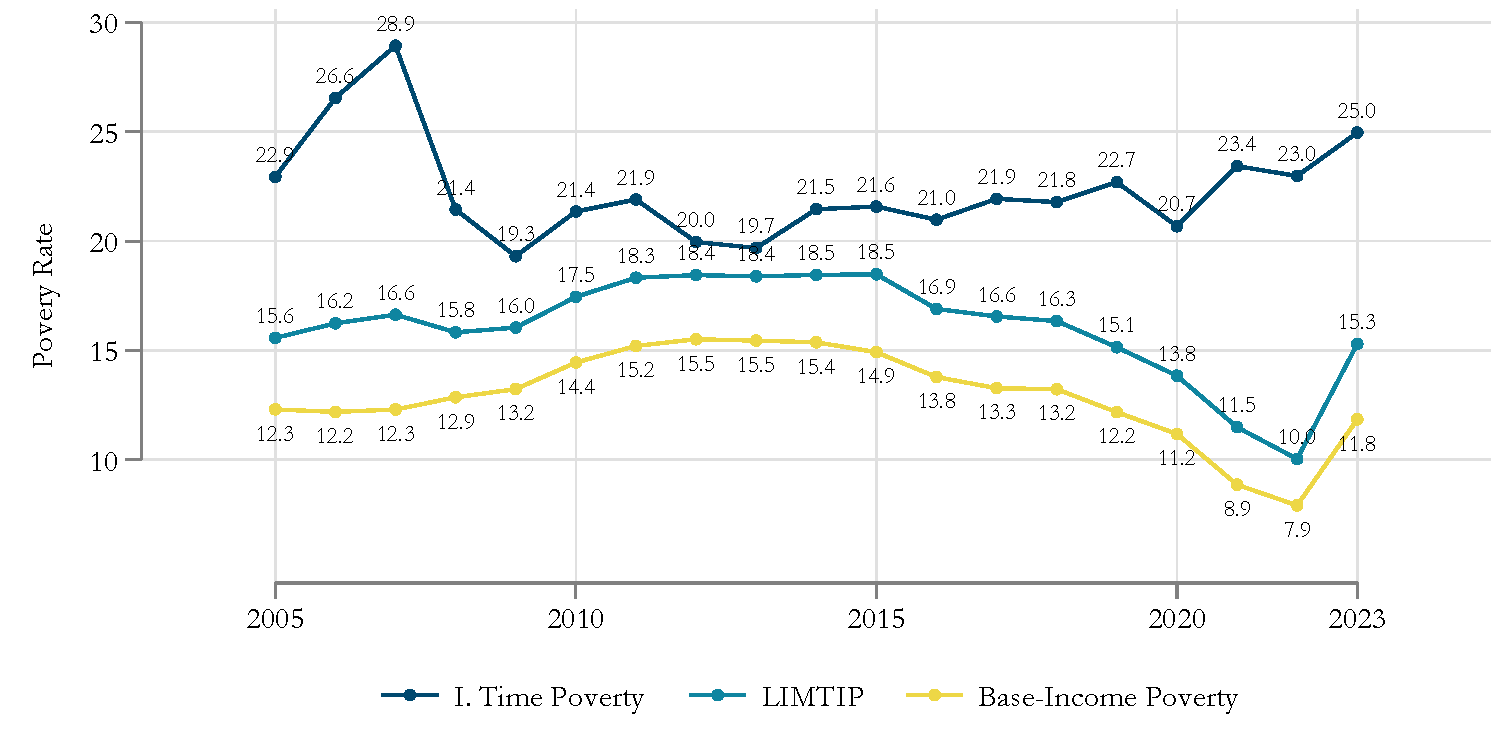
\includegraphics{resources/trend.pdf}

}

\caption{\label{fig-trend}Trends of Time, Income and Limtip Poverty in
the U.S.}

\end{figure}%

In the next section, we focus on the subsample that can potentially be
brought out of poverty.

\section{Identifying the Problem}\label{sec-problem}

One of the strategies that could help reducing the problem of time
poverty, and thereby the incidence of hidden poor, is the redistribution
of household production responsibilities across all capable (!add
footnote on capable!) members in the household. At best, household
members with time surpluses could take on more household
responsabilities, reducing the burden of those with time deficits, and
potentially bringing out household out of poverty. At worst, the
redistribution could make the time deficits more equal among the
household members, even if the household remains time poor.

Before we start analyzing the potential that redistribution could have
in reducing time poverty, we must first identify the households where
redistribution is possible and desirable. Specifically, we exclude from
the analysis households that are not time poor, even if such households
could potentially benefit from redistribution, reducing the gaps of time
surpluses among household members and even resulting in more
gender-equitable sharing of household work. From the sample of
individuals living in a time poor household we classify them into five
different groups:

\begin{itemize}
\tightlist
\item
  Single: These are time poor individuals that live in a household where
  they are the only working-age person. In this case, redistribution is
  not possible, and thus are excluded from the analysis.
\item
  Time Poor living in H. Type I: These are time poor individuals who
  live in households where all working-age members are time poor. While
  redistribution is possible, and may help in reducing the time deficits
  of individuals, and even allow some to transition out of time poverty,
  the household will remain time poor in any redistributional scenario.
\item
  Time Poor living in H. Type II: These are time poor individuals who
  live in households where there are non-time poor individuals. However,
  the combined time surpluses is insufficient to lift the household out
  of time poverty.
\item
  Time Poor living in H. Type III: These are time poor individuals who
  live in households where there is enough time surplus to lift the
  household out of time poverty. Redistribution in these households can
  lift all working members of the household out of time poverty.
\item
  Non Time poor living in a time poor household: This last group
  consists of individuals with time surpluses living in a time poor
  household. The goal of the redistribution scenarios is to allocate
  household responsabilities in such a way that these invididuals can
  help lift other household members out of time poverty. However, it is
  also possible that some of these individuals may end up experiencing
  time poverty in the redistribution scenarios. (!present this info in a
  table across columns: Red possibile or not and efficient or not/or
  what outcome it brings in, by hhtype)
\end{itemize}

Figure~\ref{fig-composition} provides a visual representation of the
classification of individuals living in time poor households. As it can
be observed, across years, about 40\% of individuals were living in a
time poor household. While this share shows a sharp increase between
2005 and 2007, it has remained stable from 2008 onwards, with a small
increase across years. There is an additional 4-5\% of individuals who
are time poor but redistribution is not possible. From the rest, about
15\% of individuals constitute our main group of analysis, i.e., those
living in households where redistribution is possible and some
individuals could benefit from it. The remaining 20\% are individuals
who are not time poor but live in a time poor household.

\begin{figure}

\centering{

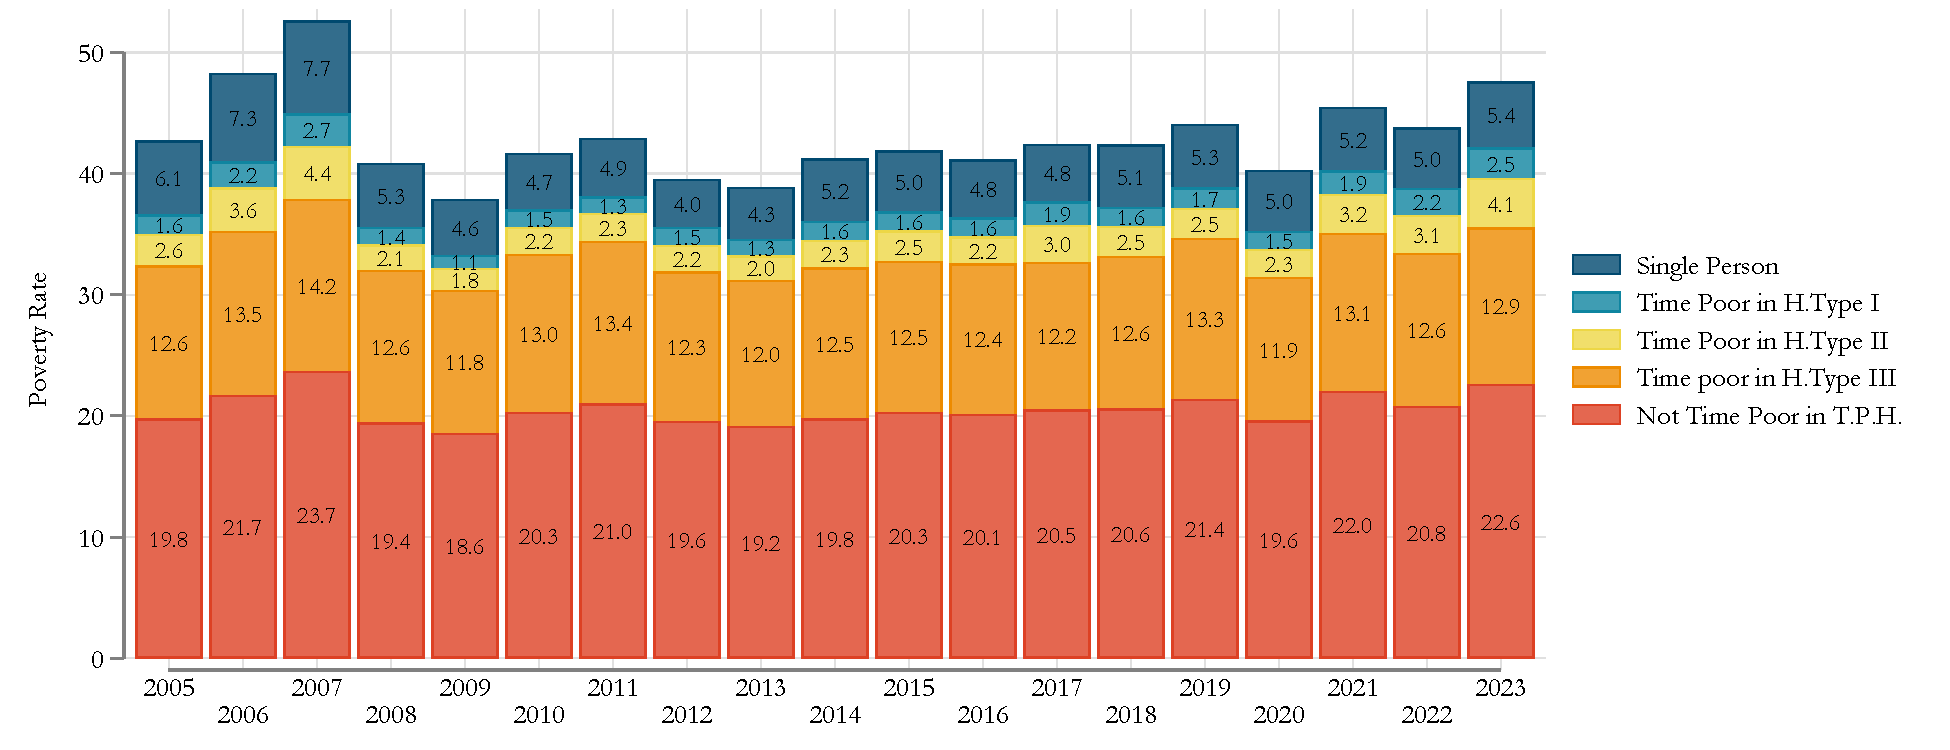
\includegraphics{resources/tpov_type.pdf}

\footnotesize 

\begin{flushleft}Note: T.P.H.= Time Poor Household, H.Type I : All working age members are time poor, H.Type II: There are Non-time poor individuals Living in the HH, but time surplus is insufficient to Lift HH out of Time poverty, H.Type III: There is enough time surplus to lift HH out of time poverty.\end{flushleft}

}

\caption{\label{fig-composition}Time Poverty classification, across
time}

\end{figure}%

In the next section, we discuss three redistribution scenarios wherein
household responsabilities can redistributed across working-age members,
under different criteria. Nevertheless, we should keep in mind that we
will only be analyzing the impact of redistribution on time poor
households with at least 2 working-age members.

\section{Redistribution Scenarios}\label{redistribution-scenarios}

\begin{itemize}
\item
  Here we would describe the three redistribution scenarios we have
  developed. This would be ``realistic'' scenarios.
\item
  Describe the scenarios and the assumptions behind them.
\end{itemize}

Intrahousehold redistribution can potentially reduce time deficits and
bring households out of poverty. We construct three redistrubution
scenarios based on different guiding principles. The extent of the
reduction would depend on the principle that we use in distributing
household responsibilities among the members. First, we use the simple
egalitarianism principle that involves an equal division of total
household productiom time among all working age members. Second, we
redistribute conditional on the time available to people. Finally, in
the thord scenario, we redsitribute based on the opportunity cost of
time for people.

We outline the methods used for implementing the scenarios, with the
detailed explanation of some aspects below.

\subsection{Distribution Rules for Household
Production}\label{distribution-rules-for-household-production}

Alternative values of \(\alpha_{ij}\) indicate how household production
requirements, net of the portion met by household members that are not
of working age or are physically unable to take on more work, are shared
among working-age people in the household. The three
scenarios/principles are:

\subsubsection{Equal Shares Scenario}\label{equal-shares-scenario}

The procedure for the equal shares scenario is relatively simple. The
shares of those in the redistribution simulation in this scenario are
simply:
\begin{equation}\phantomsection\label{eq-r1}{\alpha_{ij}^E= 1/I_j*(1-\alpha_{j}^{nw'})
}\end{equation}

where \(\alpha_{ij}\) represents the redistributed share of individual
\(i\); \(I^j\) denote the number of working-age persons in household
\(j\) and \(\alpha_{j}^{nw'}\) represents the share of non-working
group, hence \((1-\alpha_{j}^{nw'})\) representing the available
redistributable share. We count the number of people in the
redistribution simulation in each household and then assign them the
appropriate fraction (1 for households with one person in the
simulation, 1⁄2 for households with two people in the simulation, and so
on) and apply that fraction to the redistributable share of required
household production time. This scenraio overlooks time equity, i.e
redistributes without taking into consideration the time available to
individuals.

\subsubsection{Time Available Scenario}\label{time-available-scenario}

The time available scenario is based on equity such that the
redistrubted shares are based on the time that is available after
setting aside the time for personal maintenance requirements and income
generation. In other words, the household members should split up the
required household production time based on the time each one has
available, i.e based on an equity criteria. The time available
(\(Z_{ij}\)) is defined as the time left over after the minimum personal
maintenance and time spent on income generation (including commuting
time) have been subtracted from the total weekly hours. To calculate the
shares for each individual based on this principle, we first calculate
the time available for each individual, then add up the total among the
household for those individuals that have positive time available. Next,
we divide each individual's time available by the total and apply that
fraction to the redistributable share of household production time. For
those individuals that have negative time available we set their shares
to zero in this simulation.

\begin{equation}\phantomsection\label{eq-r2}{\alpha_{ij}^A= (Z_{ij}/ \sum Z_{ij}) (1-\alpha_{j}^{nw'}), if  Z_{ij}>0, 
}\end{equation}

\begin{equation}\phantomsection\label{eq-r3}{\alpha_{ij}^A =0, if Z_{ij}<0
}\end{equation}

\subsubsection{Opportunity Cost
Scenario}\label{opportunity-cost-scenario}

The third possibility is based on the idea of opportunity costs along
marginalist lines. The sharing rule depends on the relative actual
(potential) wage. For example, if there are only two working-age adults,
say husband and wife, and if the husband's wage is twice as much as the
wife, the wife's share would be two-thirds and the husband's share would
be one-third. We use the actual or shadow wage for the employed and the
potential wage for the nonemployed. Redistribution takes place based on
the following equation:
\begin{equation}\phantomsection\label{eq-r3}{\alpha_{ij}^O= (1/{I_j-1})*(1-w_{ij}/w_{ij} ) (1-\alpha_{j}^{nw'})
}\end{equation} For this simulation, we first imputed wages for all of
those not currently working for pay using a two-stage Heckman selection
model (Heckman 1979), also known as the Heckit procedure (see details
below). We them used the imputed wages of those that are not currently
working for pay and the actual wages of those that are working to divide
up the redistributable share of required household production. (!ask
FRA)

As the share of required household production needs to be inversely
proportional to the individual's share of the sum of wages, we subtract
their share of this sum from one. To ensure that the resulting shares
sum up to unity, we divide by the number of individuals in the
simulation minus one. We then apply this share to the redistributable
share of required household production as in previous steps.

In order to impute wages for those not currently employed, we first
impute the likeliest industry and occupation for each individual using a
multinomial probit procedure. Industry and occupation are regressed on
age, age squared, sex, race, education, and geographic region on all
those in the working age population (18-64). The likelihood for each
industry and occupation is then predicted for everyone, using the
results of the multinomial probit. Then each individual not currently
working for wages is assigned the industry and occupation corresponding
to the xxxx/ largest predicted likelihoods for that individual.

Next, we move on to the first stage of the Heckit procedure, a probit
estimation of a dummy variable for being employed in wage work (paid):

\begin{equation}\phantomsection\label{eq-probit}{P(paid=1|X)=F(X \beta)
}\end{equation}

where F is the cumulative density function of a normal distribution. The
vector of explanatory variables, 𝑋, comprises the individual's age, sex,
race, disability, number of kids across age groups (0 to 5, 6 to 14,
15-17), presence of spouse and spouse's age, education and employment
status education. The regression is run on the universe of all eligible
adults separately by age (divided into four categories: 18 to 30 years
old; 31 to 45 years old; and 46 to 64 years old) and sex. The Mills
ratio, 𝜆, is calculated for all individuals using the results of the
first stage regression:

\begin{equation}\phantomsection\label{eq-mills}{\lambda = f(X\beta)/ F(X\beta)
}\end{equation}

where 𝑓 and 𝐹 are, respectively, the probability and cumulative density
function of a normal distribution, and \(\beta\) is the vector of
estimated coefficients from the probit model. The second stage is an
ordinary least squares (OLS) estimate of the log of hourly wage:

\begin{equation}\phantomsection\label{eq-OLS}{lnw= (\gamma_2*Z^w) + (\theta_2 \lambda) + \mu
}\end{equation}

This regression is run only on those that are actually employed for pay
(!FRA). The vector of explanatory variables, {[}{]}, includes age, sex,
race, education, geographical region, disability, industry, occupation,
presence of spouse, spouse's employment status, and, finally, λ, the
Mills ratio calculated in the first stage. Inclusion of the Mills ratio
corrects for the selection bias induced by limiting the regression to
those in paid employment. The imputed log of wage is predicted for those
not working for wages from the results of the regression, with industry
and occupation replaced by the industries and occupations assigned in
the previous step.

We simulate each of the above principles of redistribution and
recalculate individual and household time and income poverty using the
LIMTP framework described above.

\begin{itemize}
\tightlist
\item
  Next, we provide an assessment of the different principles in terms of
  how far they improve the position of women and how much such
  improvements are congruent with the betterment of the economic
  well-being of their families. In the subsequent section, we compare
  and contrast the joint distribution of time and income poverty among
  families and individuals that would result from each principle.
\end{itemize}

\section{Results}\label{results}

As described in the previous section, we consider three scenarios to
analyze the impact that redistribution could have on time poverty,
focusing on individuals living in time poor households with at least two
working-age members. In this section, we present the results of the
redistribution scenarios and discuss the implications for time poverty
and the incidence of hidden poor. Since most of the results acrosstime
are similar, we focus on providing results that average the impacts of
redistribution across all years.

\subsection{Redistribution Scenarios and Time Poverty: General
Results}\label{redistribution-scenarios-and-time-poverty-general-results}

Figure~\ref{fig-dist} provides the distribution of individuals, and
their households by type. Figure~\ref{fig-dista} shows that 54.6\%
individuals live in time poor households are not time poor themselves.
These are the individuals that could help lift other household members
out of time poverty, by taking on more household responsibilities.

From the rest, 4.6\% live in households where everyone is time poor,
7.1\% live in households with at least one not-time-poor individual, but
with insufficient time surplus to lift the household out of time
poverty, and 33.7\% live in households where there is enough time
surplus to lift every household member out of poverty.

In terms of household structure, Figure~\ref{fig-distb} shows 81.2\% of
the households could exit from time poverty, but the remaining 18.8\%
cannot do so, even if all working-age members were to take on more
household responsibilities. Nevertheless, it may be possible to reduce
the time deficits of some individuals in these households.

\begin{figure}[H]

\centering{

\begin{figure}[H]

\begin{minipage}{0.50\linewidth}

\centering{

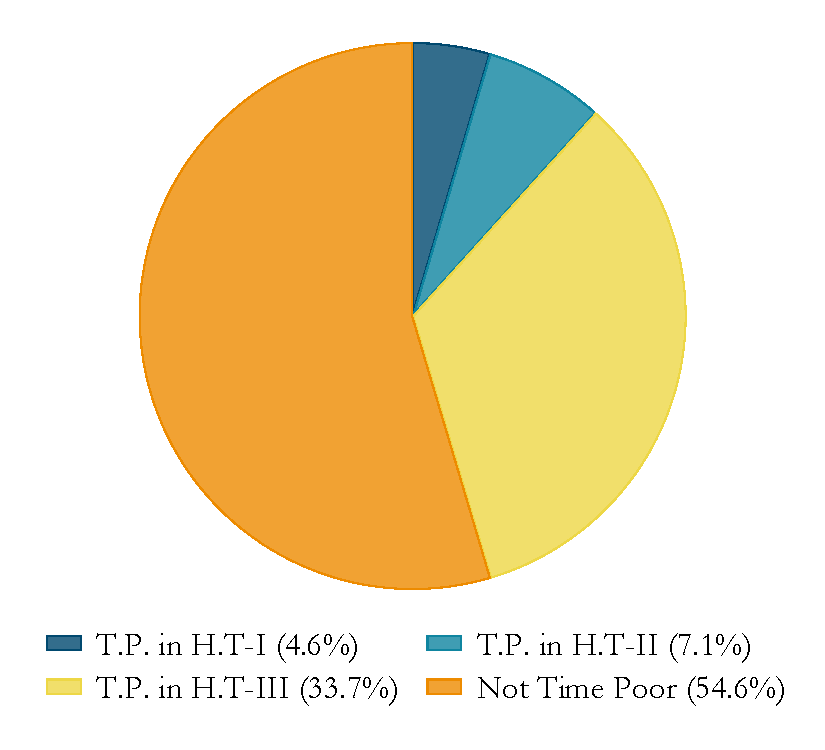
\includegraphics{resources/ind_dist.pdf}

}

\subcaption{\label{fig-dista}Individuals}

\end{minipage}%
%
\begin{minipage}{0.50\linewidth}

\centering{

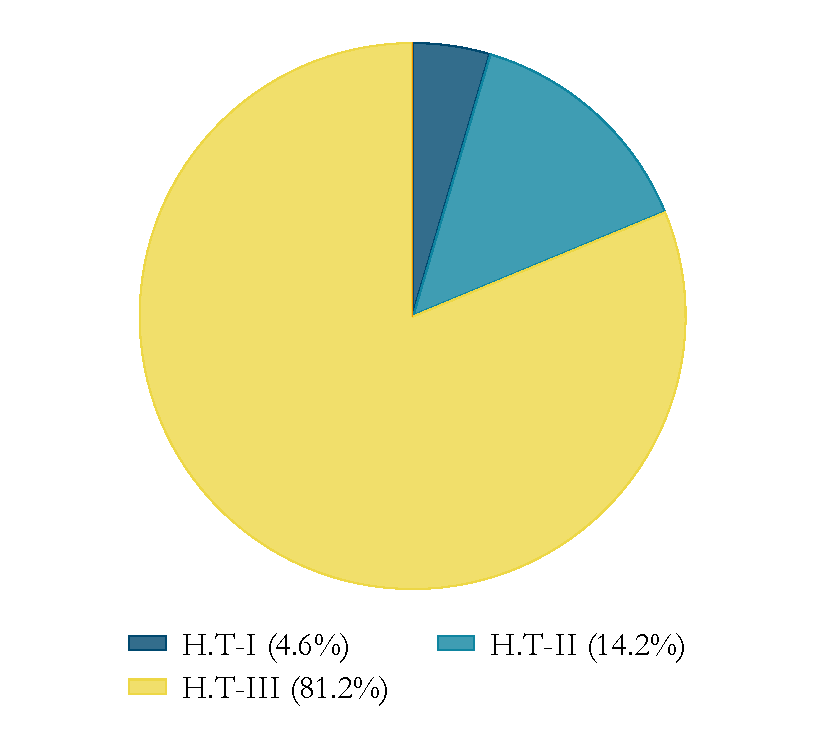
\includegraphics{resources/hh_dist.pdf}

}

\subcaption{\label{fig-distb}Households}

\end{minipage}%

\end{figure}%

\footnotesize 

\begin{flushleft}Note: H.Type I : All working age members are time poor, H.Type II: There are Non-time poor individuals Living in the HH, but time surplus is insufficient to Lift HH out of Time poverty, H.Type III: There is enough time surplus to lift HH out of time poverty.\end{flushleft}

}

\caption{\label{fig-dist}Distribution of individuals by type}

\end{figure}%

To understand the impact of the diferent redistribution scenarios on
these groups, we will focus on transition probabilities, focusing on
individual experiences first. For individuals who are currently not time
poor, the statistic of interest would be the likelihood that they fall
into time poverty, whereas for time poor individuals, we will consider
their porverty exit rate.

\begin{figure}[H]

\centering{

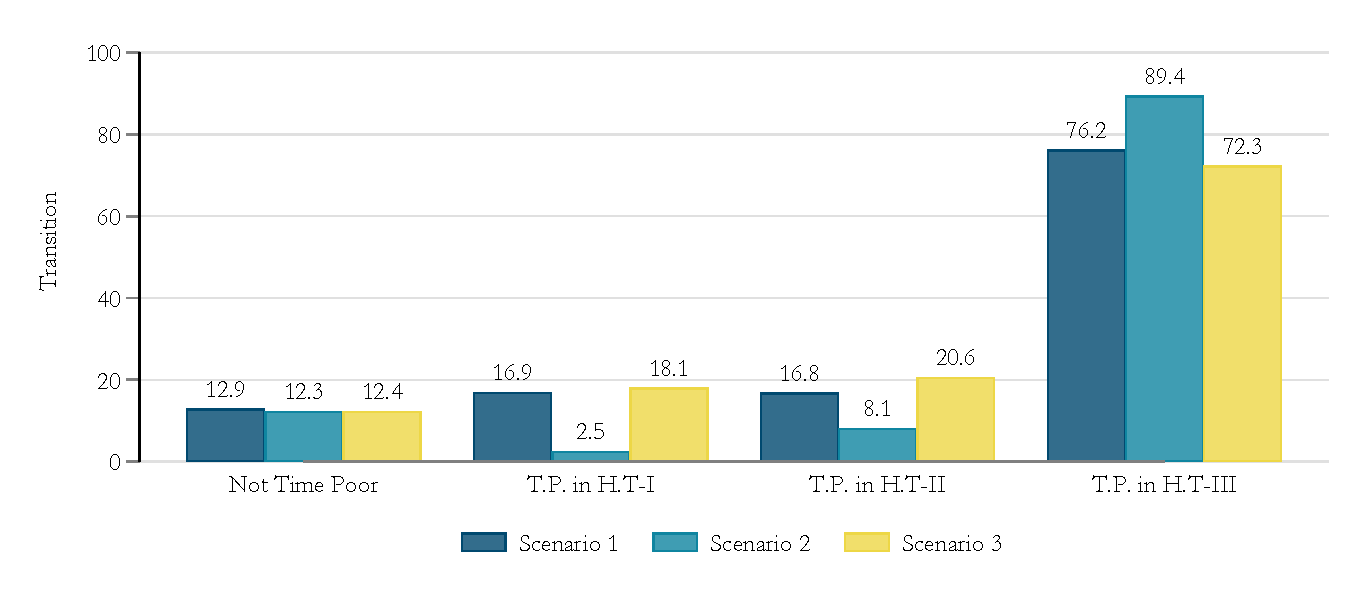
\includegraphics{resources/trans1.pdf}

}

\caption{\label{fig-transition1}Transition probabilities by
Redistribution Scenario}

\end{figure}%

As observed in Figure~\ref{fig-transition1}, because the all
redistribution scenarios are designed to redistribute household
production responsibilities, without avoiding putting some individuals
in time poverty, there is a 12.3-12.9\% probability that non time poor
individuals will fall into time poverty. While this probabilities is
considerably similar across scenarios, its not the same individuals that
are affected (see Figure~\ref{fig-tran_by_group1} and
Figure~\ref{fig-tran_by_group2}).

In terms of time Deficits, the average time deficits that non-time poor
individuals face is quite small, just around 0.7 hours. However, those
who become time poor increase their time deficits to around 4.4-5.8hrs
per week. Interestingly, the Time availability Scenario (Scenario 2) has
the lowest impact in terms of time deficits for this subgroup.

For the rest of the categories, we observe that there are substantially
more heterogeneity on the impact of time povery across the different
Scenarios. For individuals in households where all members are time
poor, the equal share and opportunity cost scenarios suggest that up to
17\%-18\% of individuals could exist time poverty, with only a 2.5\%
exit rate under the time availability scenario.

While such case may suggest an improvement on the quality of life of
some individuals, the redistribution scenarios also have implications in
terms of time deficits other household members face. As shown in
Figure~\ref{fig-def1}, average time deficit increase in roughly 1 hour
for scenarios 1 and 3. However, as shown in Figure~\ref{fig-def2}, the
time deficit for those who remain time poor increase in just over 3hrs.
In general, while the availability scenario has smallest impact on
transition rates, it also has the smallest impact in terms of time
deficits, for those who remain time poor.

\begin{figure}[H]

\centering{

\centering{

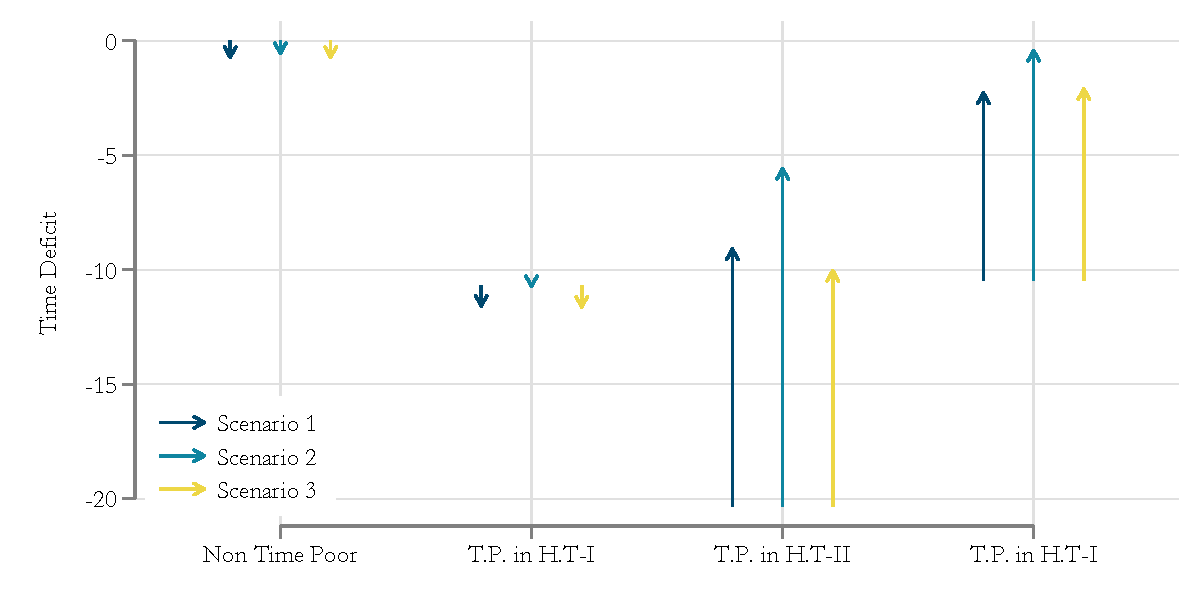
\includegraphics{resources/def1.pdf}

}

\subcaption{\label{fig-def1}Average Time Deficits}

\centering{

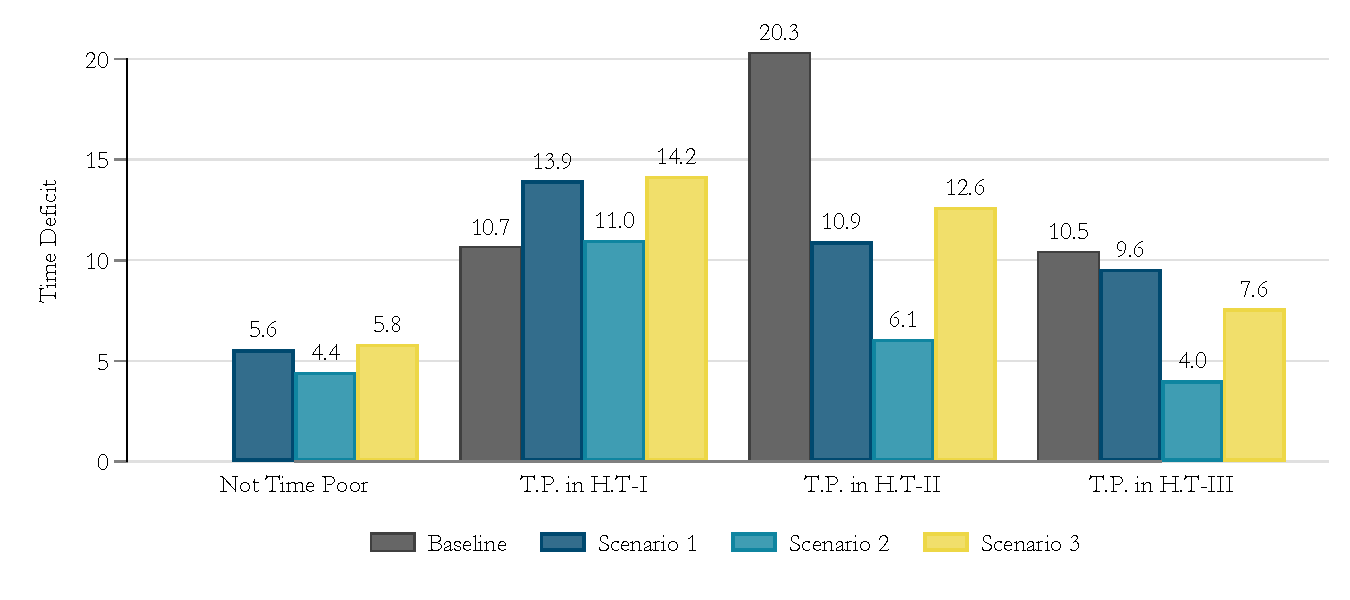
\includegraphics{resources/def2.pdf}

}

\subcaption{\label{fig-def2}Average Time Deficits (Excluding Zeros)}

}

\caption{\label{fig-deficit}Time Deficits across Scenarios}

\end{figure}%

The next group of interest are those individual living in households
that cannot exit time poverty, but could reduce time deficits for some
of their members (Household Type II). Interestingly, the poverty exit
rates for these individuals are ver similar as for the previous group,
with the time availability scenario having the lowest impact at 8.1\%.
In contrast, when we pay attention to the time deficits, its the equal
share scenario that has the largest impact on time deficit.

At baseline, individuals in this group had in average a time deficit of
20hrs per week. Under Scenarios 1 and 3, the average deficit reduces to
9hrs and 10hrs respectively. However, under Scenario 2, it reduces to
only 5.6hrs a week. While the time availability scenario is not as
effective in reducing time poverty, it may appear it is the most fair,
as it redistributes both the gains and losses of time allocation more
equally across household members.

The last group of interest are those individuals living in households
where redistribution could lift all members out of time poverty. In this
case, all redistribution scenarios do an excellent job at reducing time
poverty, with exit rates of 72-89\%. In contrast with the two previous
cases, the time availability scenario has the largest impact reducing
time poverty, with an exit rate of 89\%. In terms of time deficits,
given the success the redistribution scenarios have in reducing time
poverty, the average time deficits is reduced to 0.4-2.3hrs per week.
However, for those who remain time poor, the impacts in terms of time
deficits are much smaller, with scenario 2 still representing the most
efficient, reducing the deficit to just 4hrs per week.

As it would be expected, this reduction in individual time poverty also
has an impact at the household. While non of the households Type I or II
are able exit time poverty, as shown in Figure~\ref{fig-transition2},
between 65-87\% of households Type III are able to exit time poverty,
with Scenario 2 being the best at reducing time poverty.

\begin{figure}[H]

\centering{

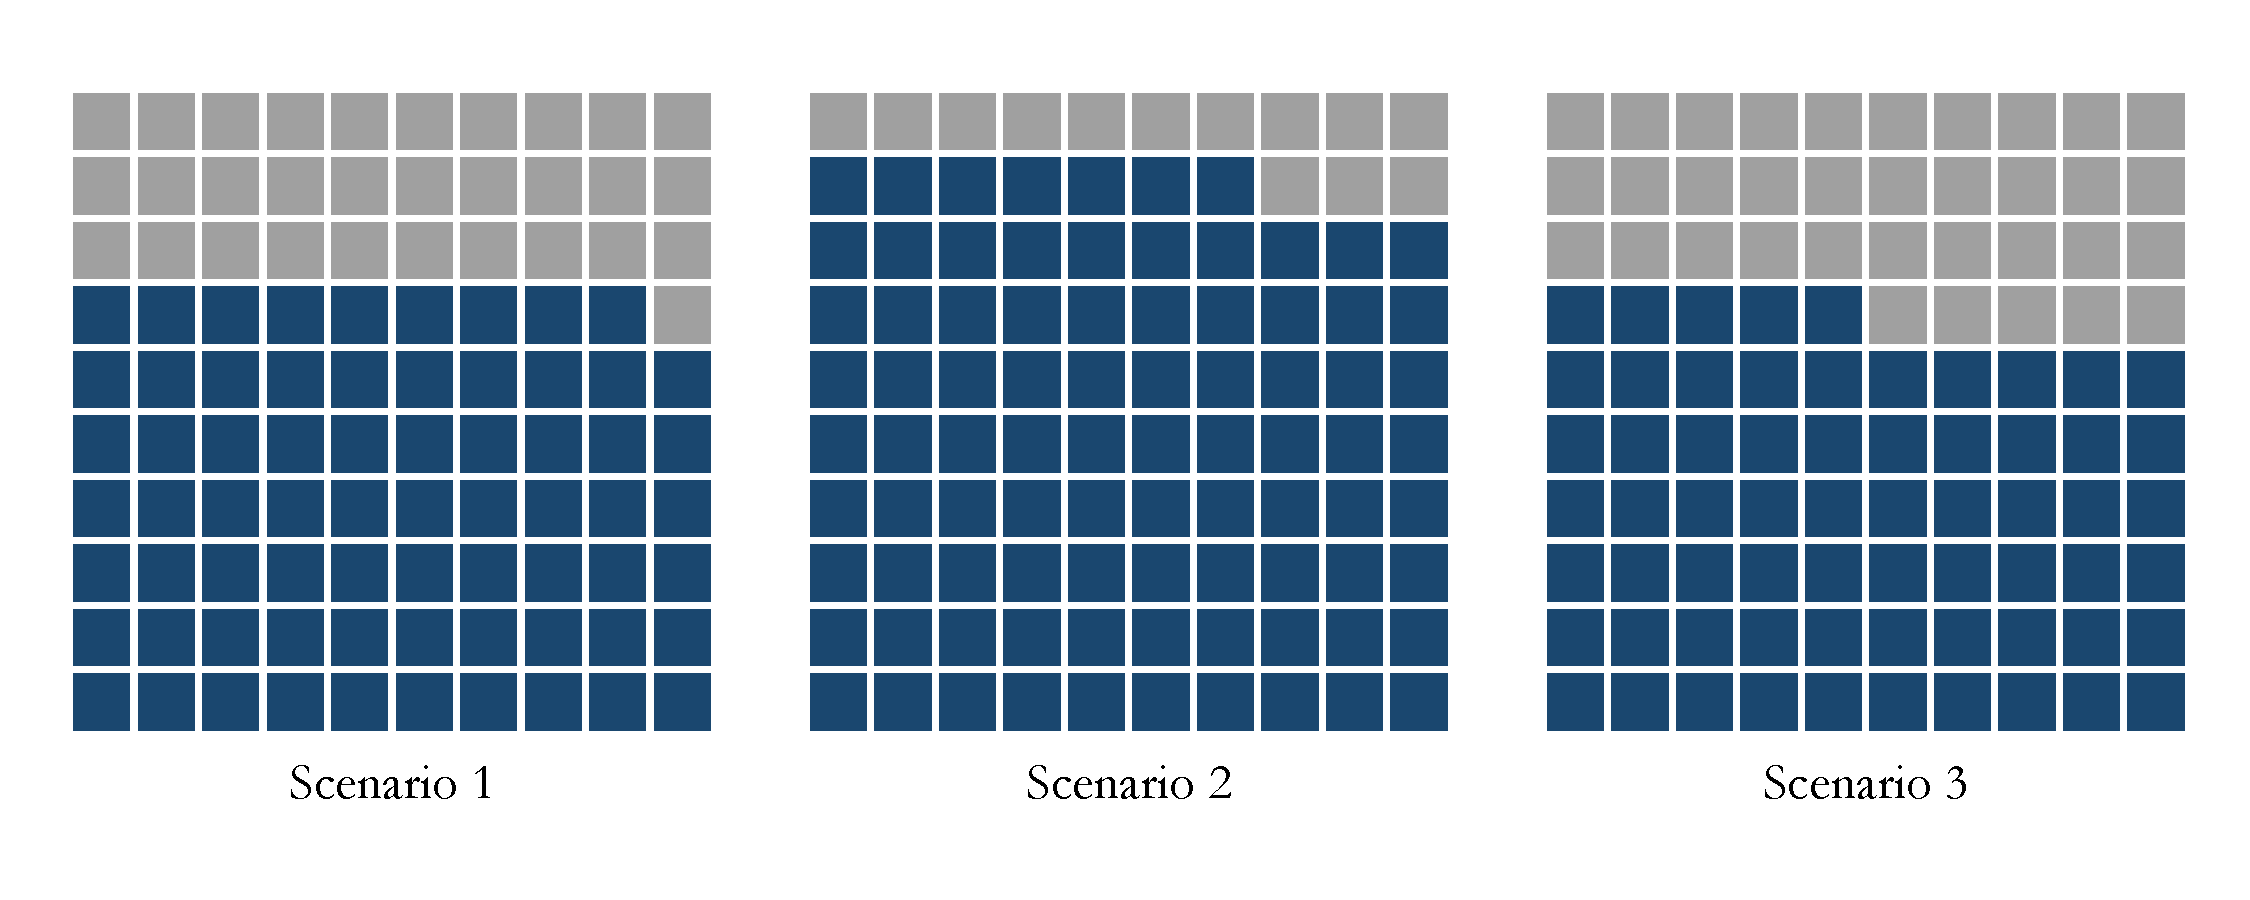
\includegraphics[width=0.7\textwidth,height=\textheight]{resources/hhtrans.pdf}

}

\caption{\label{fig-transition2}Transition probabilities for households}

\end{figure}%

\subsection{Redistribution Scenarios and Time Poverty:
Heterogeneity}\label{redistribution-scenarios-and-time-poverty-heterogeneity}

As suggested earlier, not all individuals were affected in the same way
by the redistribution scenarios. For example, groups who are
traditionally more vulnerable to time poverty, are also the most likely
to benefit from intra household redistribution of responsabilities. To
explore this further, in this section we present how the poverty
transition rates varies across different groups of individuals.
Figure~\ref{fig-tran_by_group1} and Figure~\ref{fig-tran_by_group2}
present the difference between the group specific transition rate
compares to the overall transition rate.

Under Scenarios 1 and 2, men have a higher probability of falling into
time poverty compared to women, with a lower probability of exiting time
poverty. This is particularly pronouced among individuals living in
type-III households. Interestingly, Scenario 3, which is based on
opportunity costs, shows the opposite pattern. Although we have shown
that all scenarios help reduce time poverty, the opportunity cost
scenario seem to attenuate the effect by perpetuating the gender roles
tied to earning potentials.

A second characteristics that tends to drive differences in time poverty
is related to the presence of Children. In our results, however, their
presence has mixed impact oon tn transition rates. Under all scenarios,
not time poor individuals living in households with children are more
like to fall into time poverty. However having children also increases
the chances of exiting time poverty in Household Type II, while reducing
it in Household Type III. The time availability scenario is the only
case where the results are consistent across all household types, with
children increasing the probability of falling into time poverty, but
decreasing the probability of exiting time poverty.

The last group of interst considered in Figure~\ref{fig-tran_by_group1}
is based on employment status. Since time poverty is closely related to
the time spent on paid work, we should emphasize that the share of time
poor individuals among the not employed is much smaller compared to the
employed. Because of this, the unemployed have an almost 0\% probability
of falling into time poverty, and those who are time poor, are far more
likely exit time poverty. Among the employed, while they are somewhat
more likely to fall into time poverty than average, there are almost no
singificant differences in any other scenario.

\begin{figure}[H]

\centering{

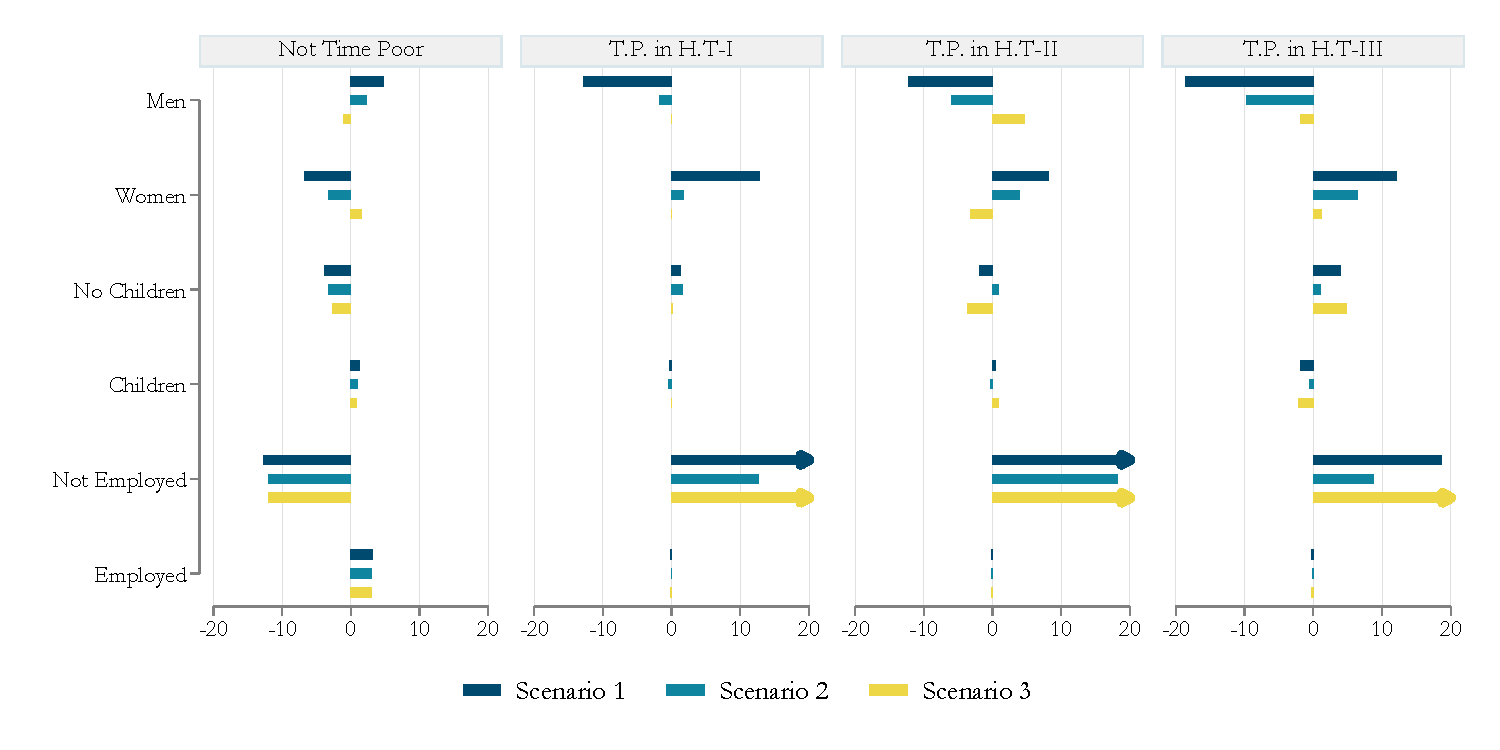
\includegraphics{resources/det1.pdf}

\footnotesize 

\begin{flushleft}Note: The figure presents the difference between the group specific transition rate and the overall transition rate.\end{flushleft}

}

\caption{\label{fig-tran_by_group1}Transition probabilities
Heterogeneity: Gender, Employment Status and Children Presence}

\end{figure}%

In terms of education and age (see Figure~\ref{fig-tran_by_group2}) the
patterns are less clear. Among non time poor individuals, those with
higher levels of education seem to be the most likely to fall into time
poverty. This pattern is observed for all scenarios, with but with a
smaller impact under the opportunity cost scenario.

For time poor individuals, the patterns are less clear. When
redistribution is driven by oppotunity cost, higher levels of education
increase the probability of exiting time poverty. However, the magnitude
of the diferences is small for type III households. For Scenarios 1 and
2, we can only observe some patterns for individuals living in type III
households, where higher education reduce, rather than increase, the
probability of exiting time poverty.

Finally, in terms of age, both the youngest and oldest individuals are
less likely to fall into poverty, while also being the more likely to
exit time poverty. This patterns may be a reflection that individuals in
the age group 30-45 are most likely to be in the labor market, and thus
are less flexible in terms of time allocation, and thus are less likely
to be affected by the redistribution scenarios.

\begin{figure}[H]

\centering{

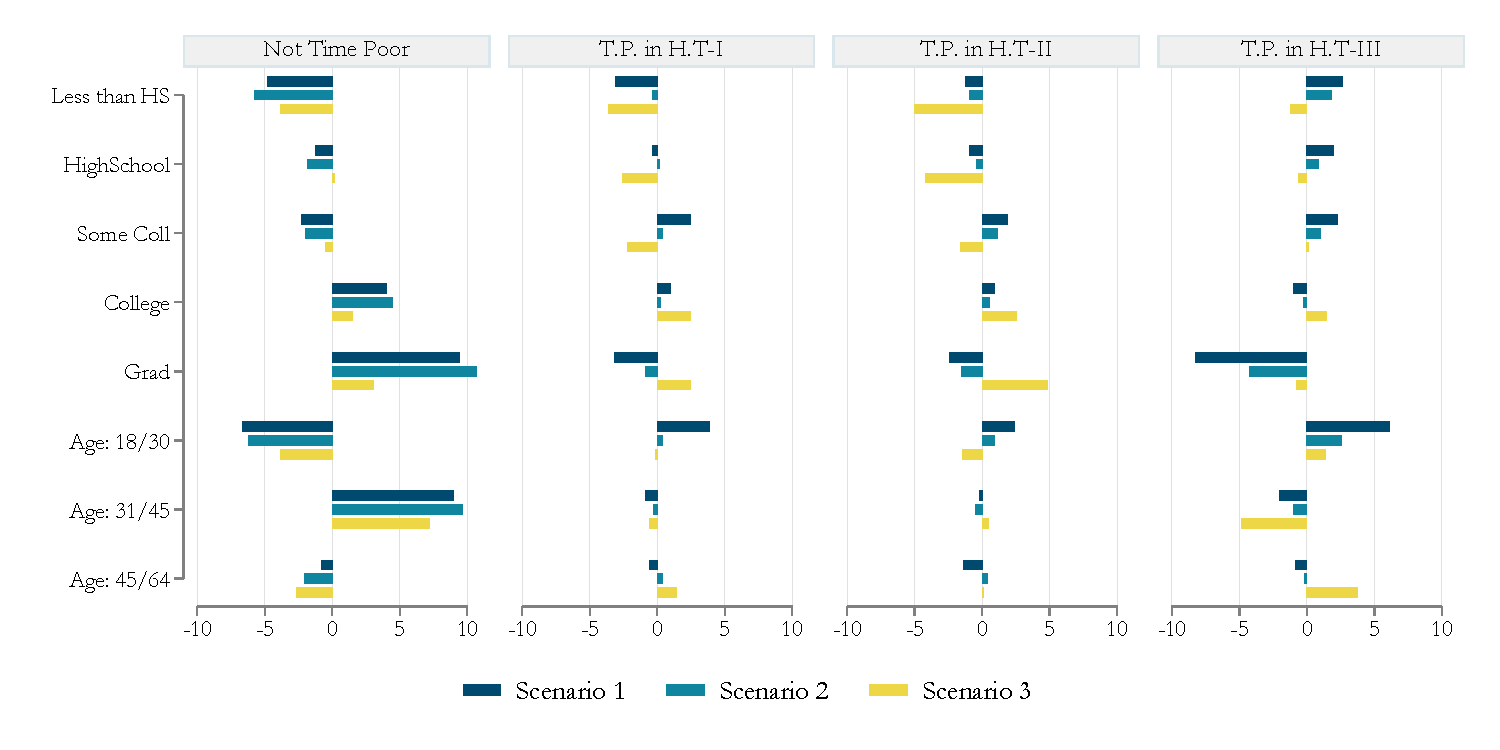
\includegraphics{resources/det2.pdf}

\footnotesize 

\begin{flushleft}Note: The figure presents the difference between the group specific transition rate and the overall transition rate.\end{flushleft}

}

\caption{\label{fig-tran_by_group2}Transition probabilities
Heterogeneity: Education and Age}

\end{figure}%

\subsection{Changes in LIMTIP: The hidden
poor}\label{changes-in-limtip-the-hidden-poor}

WHile the discussion above provides a detailed picture of the potential
impact that redistribution could have on time poverty, it is equally
important to understand changes in terms of Adjusted LIMTIP estimates.

\begin{figure}[H]

\centering{

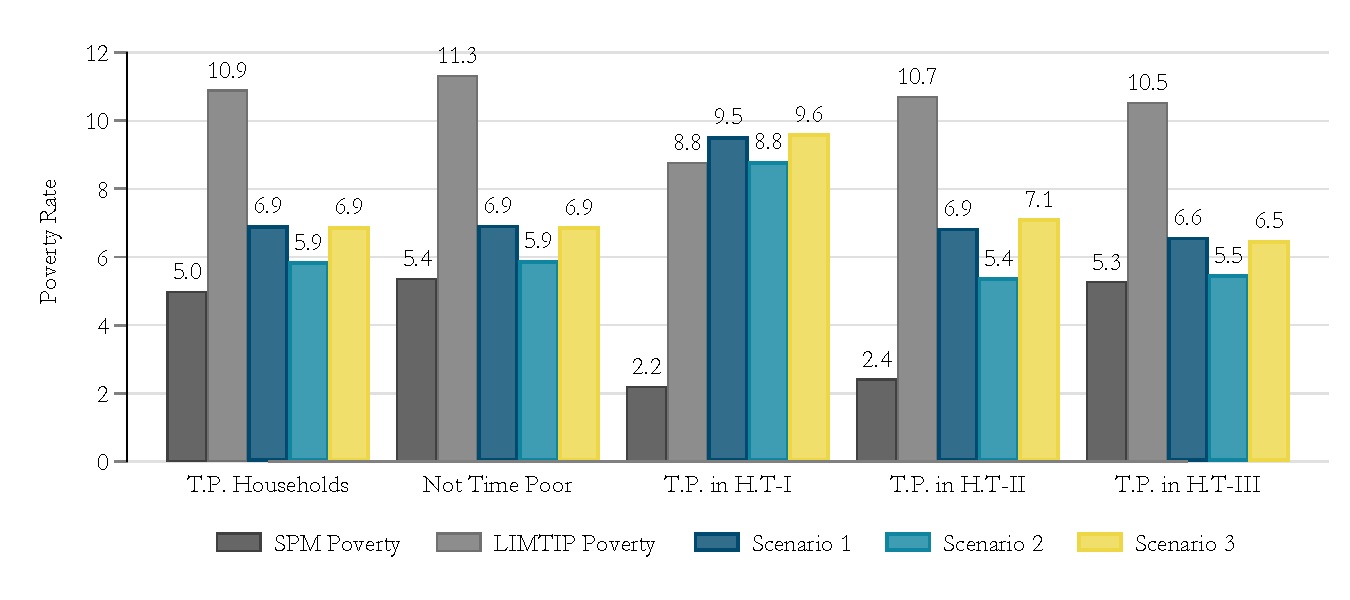
\includegraphics{resources/glimtip.pdf}

}

\caption{\label{fig-limtip}Changes in LIMTIP estimates across
redistribution scenarios}

\end{figure}%

In Figure~\ref{fig-limtip} we present the poverty rates across the
different redistribution scenarios, for the sample of households that we
identify to be time poor. The first thing to consider here is that the
incidence of official poverty and LIMTIP poverty in the sample is lower
than the one observed in the general population
(Figure~\ref{fig-trend}). This is expected, since our sample of
interested is restricted to time poor households, who are more likely to
have members working, and hence less likely to be income poor.

Even in this sample we observe a large difference between the official
poverty estimates and the LIMTIP estimates. While the official poverty
estimates are around 5\%, the LIMTIP estimates poverty to be closer to
11\%, showing that 6\% of the individuals in the sample are hidden poor.
Given the success of the redistribution scenarios in reducing time
poverty, we observe that the LIMTIP estimates are also reduced, with the
time availability scenario showing the largest reduction in poverty
rates, practically eliminating the incidence of hidden poor in the
sample.

However, a detailed look across individuals suggests that such large
improvements are not uniform across all groups. In households where all
individuals are time poor, the redistribution scenarios worsen the
poverty rates, albeit the impact is small. This happens because the
aggregated time deficit of the household increases as some individuals
who exit time poverty status. For households with some potential to
reduce aggregated time deficits (H.Type II), we observe that the share
of the hidden poor is greatly reduced from 8\% to 3 to 5\%.

\section{Policy implications}\label{policy-implications}

\section{Conclusion}\label{conclusion}

\section*{References}\label{sec-ref}
\addcontentsline{toc}{section}{References}

\phantomsection\label{refs}
\begin{CSLReferences}{1}{0}
\bibitem[\citeproctext]{ref-berik2009}
Berik, G., Rodgers, Y. van der M., and Seguino, S. (2009). Feminist
{Economics} of {Inequality}, {Development}, and {Growth}. \emph{Feminist
Economics}, \emph{15}(3), 1--33.
\url{https://ezprox.bard.edu/login?url=https://search.ebscohost.com/login.aspx?direct=true&db=ecn&AN=1063369&site=eds-live&scope=site}

\bibitem[\citeproctext]{ref-hundt1996}
Bruyn-Hundt, M. (1996). Scenarios for a redistribution of unpaid work in
the netherlands. \emph{Feminist Economics}, \emph{2}(3), 129--133.
\url{https://doi.org/10.1080/13545709610001707826}

\bibitem[\citeproctext]{ref-duflo2012}
Duflo, E. (2012). Women {Empowerment} and {Economic} {Development}.
\emph{Journal of Economic Literature}, \emph{50}(4), 1051--1079.
\url{https://doi.org/10.1257/jel.50.4.1051}

\bibitem[\citeproctext]{ref-elson2017}
Elso, D. (2017). \emph{Recognize, {Reduce}, and {Redistribute} {Unpaid}
{Care} {Work}: {How} to {Close} the {Gender} {Gap}}.
\url{https://doi.org/10.1177/1095796017700135}

\bibitem[\citeproctext]{ref-elson2009}
Elson, D. (2009). Gender {Equality} and {Economic} {Growth} in the
{World} {Bank} {World} {Development} {Report} 2006. \emph{Feminist
Economics}, \emph{15}(3), 35--59.
\url{https://doi.org/10.1080/13545700902964303}

\bibitem[\citeproctext]{ref-valeria2016}
Esquivel, V. (2016). Power and the {Sustainable} {Development} {Goals}:
A feminist analysis. \emph{Gender \& Development}, \emph{24}(1), 9--23.
\url{https://doi.org/10.1080/13552074.2016.1147872}

\bibitem[\citeproctext]{ref-hess2020}
Hess, Cynthia, Ahmed, T., and Hayes, J. (2020). \emph{Providing {Unpaid}
{Household} and {Care} {Work} in the {United} {States}: {Uncovering}
{Inequality}}.

\bibitem[\citeproctext]{ref-malik2018}
Malik, R., Hamm, K., Schochet, L., Novoa, C., Workman, S., and
Jessen-Howard, S. (2018). America's {Child} {Care} {Deserts} in 2018.
\emph{Center for American Progress}.
\url{https://www.americanprogress.org/article/americas-child-care-deserts-2018/}

\bibitem[\citeproctext]{ref-oecd2020}
OECD. (2020). \emph{Early learning and child well-being in the united
states} (p. 124).
https://doi.org/\url{https://doi.org/https://doi.org/10.1787/198d8c99-en}

\end{CSLReferences}



\end{document}
